%%%%%%%%%%%%%%%%%%%%%%%%%%%%%%%%%%%%%%%%%%%%%%%%%%%%%%%%%%%%%%%%%%%%%%%%%%%%%%%%
%     Escape rate for a Brownian particle in a radial cubic spline trap        %
%                           Marc Meléndez Schofield                            %
%%%%%%%%%%%%%%%%%%%%%%%%%%%%%%%%%%%%%%%%%%%%%%%%%%%%%%%%%%%%%%%%%%%%%%%%%%%%%%%%

%%%%%%%%%%%%%%%%%%%%%%%%%%%%%%%%%%%% Head %%%%%%%%%%%%%%%%%%%%%%%%%%%%%%%%%%%%%%

\documentclass{article}
\usepackage[utf8]{inputenc}
\usepackage{amsmath}
\usepackage{comment}
\usepackage{graphicx}
\usepackage{listings}
\usepackage{hyperref}

\title{Escape rate for a Brownian particle in a radial cubic spline trap}
\author{Marc Meléndez}

%%%%%%%%%%%%%%%%%%%%%%%%%%%%%%%%%%%% Body %%%%%%%%%%%%%%%%%%%%%%%%%%%%%%%%%%%%%%

\begin{document}

\maketitle

%! codeblock: introduction
Brownian motion has many applications in mathematics, physics and finance, but
it was originally conceived as the description of small micron-scale particles
suspended in water, which vibrate due to thermal fluctuations. Here, we are
interested in a Brownian particle that moves around in two dimensions and feels
the force due to a particular type of potential energy trap. We aim to describe
the time it takes for such a particle to escape from the trap.
%! codeblockend

\section{Cubic spline trap}

Let $r$ represent the distance between the position of a Brownian particle and
the centre of a cubic spline trap, and let $V(r)$ represent the potential energy
of such a particle (see Fig. \ref{cubic_spline}). We choose $V(r)$ in such a way
that the depth of the trap equals $E_0$, its radius is $R$ and, that it lies
flat at the origin and at $r = R$ (so $V'(0) = V'(R) = 0$).
\begin{equation}
  V(r) =
  \begin{cases}
    E_0 \left(-2\left(\frac{r}{R}\right)^3
              + 3 \left(\frac{r}{R}\right)^2 - 1\right), & \text{for } r < R, \\
    0, & \text{for } r \geq R.
  \end{cases}
\end{equation}
A trapped particle, then, feels a force
\begin{equation}
  \mathbf{F}(\mathbf{r}) = -\nabla V
                         = \frac{6}{R^2}
                           \left(\frac{r}{R} - 1\right)\ \frac{\mathbf{r}}{R}.
\end{equation}

\begin{comment}
This gnuplot code produces a graph of $V(r)$, used in the figure below.
%! codefile: cubic_spline.gnuplot
set term postscript eps enhanced size 7cm,4cm font "Roman"
set output "cubic_spline.eps"
set xlabel "{/:Italic r / R}"
set ylabel "{/:Italic V}({/:Italic r/R}) {/:Italic / E}_0"
plot [0:1.5][-1.2:0.2] (x<1)?-2*x**3 + 3*x**2 - 1:0 w l lw 3 lc -1 notitle, \
                       0 w l lc -1 dt 2 notitle
%! codeend
\end{comment}

\begin{figure}
  \centering
  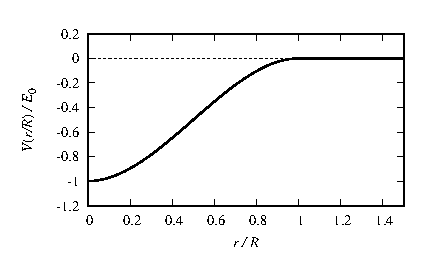
\includegraphics[width=\linewidth]{cubic_spline.eps}
  \caption{\label{cubic_spline}Radially symmetrical cubic spline trap of depth
           $E_0$.}
\end{figure}

We wish to determine the rate at which a trapped Brownian particle escapes from
the trap. Dimensional analysis reveals that the rate $\mu$ equals
\begin{equation}
\label{dimensional_analysis}
  \mu = \frac{D}{R^2}\ f\left(\frac{E_0}{k_BT}\right),
\end{equation}
where $D$ stands for the diffusion coefficient, $k_BT$ the thermal energy, and
$f$ for an as yet undetermined function.

\section{Numerical simulation}

We can check our predictions by setting up a numerical simulation of the process
process. A minimal C program could accept $E_0$, $R$, $D$ and $k_BT$ as
parameters.

\lstset{language = c, morecomment = [is]{\%!}{\^^M}}
\begin{lstlisting}[frame=single]
%! codeblock: usage_message
  /* Usage message */
  if(argc < 6) {
    fprintf(stderr, "Usage: %s <trap depth> "
                              "<trap radius> "
                              "<diffusion coefficient> "
                              "<thermal energy>"
                              "<dim>\n",
            argv[0]);
    return 0;
  }
%! codeblockend
\end{lstlisting}


\begin{comment}
%! codefile: cubic_spline.c
# include <stdio.h>
# include <stdlib.h>
# include <math.h>
# include "random.h"

int main(int argc, char * argv[])
{
  %! codeinsert: usage_message

  %! codeinsert: variable_declarations

  %! codeinsert: Brownian_simulation

  %! codeinsert: output_results

  return 0;
}
%! codeend
\end{comment}

Following the usage message, we declare the parameters and variables needed for
the Brownian simulation. The jagged trajectory of Brownian motion results from
integrating the (It\=o) stochastic differential equation
\begin{equation}
  d\mathbf{r} = M \mathbf{F}(\mathbf{r})\ dt + \sqrt{2 D}\ d\mathbf{W},
\end{equation}
where $M = D/k_BT$ stands for the particle mobility, $-\nabla V$ is the force
due to our cubic spline trap and $d\mathbf{W}$ is the two-dimensional Wiener
process.

\begin{lstlisting}[frame=single]
%! codeblock: variable_declarations
  /* Simulation parameters */
  double E0 = atof(argv[1]); /* Trap depth */
  double R = atof(argv[2]);  /* Trap radius */
  double D = atof(argv[3]);  /* Diffusion coefficient */
  double kT = atof(argv[4]); /* Thermal energy */
  int dim = atoi(argv[5]);   /* Dimensionality */
  double M = D/kT;           /* Mobility */
  double dt = 0.0001;        /* Time step */

  /* Variable declarations */
  int nruns = 10000;    /* Number of runs */
  int run;              /* Current run */
  int i;                /* Coordinate index */
  double q[dim];        /* Particle position */
  double F[dim], Fmod;  /* Force and modulus of force*/
  double r;             /* Distance to origin */
  double r2;            /* Distance squared */
  long int tstep;       /* Current step */
  long int sumtime = 0; /* Sum of times */
  long int sumt2 = 0;   /* Sum of times squared */
%! codeblockend
\end{lstlisting}

The \texttt{nruns} realisations of the stochastic process proceed by setting the
Brownian particle at the origin of coordinates and then letting it diffuse until
it reaches the edge of the trap at $r = R$. An Euler-Maruyama scheme integrates
the equations of motion. \texttt{Gaussian(0,1)} produces a random number from a
normal distribution with null mean and unit standard deviation.

\begin{lstlisting}[frame=single]
%! codeblock: Brownian_simulation
  /* nruns realisations of the stochastic process */
  for(run = 0; run < nruns; run++) {
    /* Reset position */
    for(i = 0; i < dim; ++i) q[i] = 0.0;

    /* Run Brownian dynamics until particle escapes */
    for(tstep = 0; 1; tstep++) {
      /* Particle position */
      r2 = 0; for(i = 0; i < dim; ++i) r2 += q[i]*q[i];
      r = sqrt(r2);

      /* Break when particle leaves the trap */
      if(r >= R) break;

      /* Force vector */
      Fmod = 6.0*E0*(r/R - 1)/(R*R*R);
      for(i = 0; i < dim; ++i) F[i] = Fmod*q[i];

      /* Euler-Maruyama scheme */
      for(i = 0; i < dim; ++i)
        q[i] += M*F[i]*dt + Gaussian(0,1)*sqrt(2*D*dt);
    }

    sumtime += tstep;
    sumt2 += tstep*tstep;
  }
%! codeblockend
\end{lstlisting}

The code ends by outputting the results, calculating the inverse of the mean
time it took the Brownian motion to escape from the trap.

\begin{lstlisting}[frame=single]
%! codeblock: output_results
  float meantime = (sumtime*dt)/((float) nruns);
  float mu = 1.0/meantime;

  printf("# E0 \t\t R \t\t D \t\t kT \t\t "
         "mu \t\t error(mu)\n");
  printf("%f\t%f\t%f\t%f\t%f\t%f\n", E0, R, D, kT, mu,
          mu*mu*sqrt((sumt2*dt*dt)/((float) nruns)
                     - meantime*meantime)/sqrt(nruns));
%! codeblockend
\end{lstlisting}


\section{Numerical results}

The first very obvious test of the code verifies that $\mu$ is indeed
proportional to $D$ and inversely proportional to $R^2$, as stated by Eq.
(\ref{dimensional_analysis}). Fig. \ref{mu_vs_D_and_R} shows that the
simulations agree with this prediction, although smaller values of $R$
depart from the curve, probably due to issues with the integration time
step.

\begin{comment}
With an operating cubic_spline program, we can easily generate the data files
using a bash script.
%! codefile: cubic_spline.sh
#!/bin/bash
echo "Running simulations to create data files. This will take fairly long..."
for D in `seq 0.2 0.2 2`; do ./cubic_spline 1 1 $D 1 2; done | grep -v "#" > mu_vs_D.dat
for R in `seq 1 0.2 3`; do ./cubic_spline 1 $R 1 1 2; done | grep -v "#" > mu_vs_R.dat
for E0 in `seq 0.25 0.25 7.5`; do ./cubic_spline $E0 1 1 1 2; done | grep -v "#" > mu_vs_E0.dat
for E0 in `seq 0.25 0.25 7.5`; do ./cubic_spline $E0 1 1 1 1; done | grep -v "#" > mu_vs_E0_1D.dat
%! codeend

The next figure plots $mu$ versus D and R to check the validity of Eq.
(\ref{Dimensional analysis}).

%! codefile: mu_vs_D_and_R.gnuplot
set term postscript eps enhanced size 8cm,4cm font "Roman"
set output "mu_vs_D_and_R.eps"
set ylabel "{/Symbol m} [a.u.]"
set size square

f(x) = a*x
fit f(x) "mu_vs_D.dat" u 3:5 via a
g(x) = b/(x**2)
fit g(x) "mu_vs_R.dat" u 2:5 via b

set multiplot layout 1,2
set xlabel "{/:Italic D} [a.u.]"
plot [0:2][0:6] "mu_vs_D.dat" u 3:5:6 w errorbars notitle lc -1, \
                f(x) w l dt 2 lc -1 notitle
set xlabel "{/:Italic R} [a.u.]"
plot [0:3][0:5] "mu_vs_R.dat" u 2:5:6 w errorbars notitle lc -1, \
                g(x) w l dt 2 lc -1 notitle
unset multiplot
%! codeend
\end{comment}

\begin{figure}
  \centering
  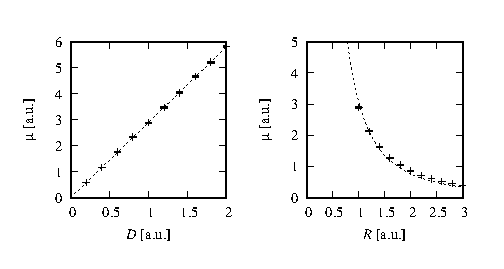
\includegraphics[width=\linewidth]{mu_vs_D_and_R.eps}
  \caption{\label{mu_vs_D_and_R}Escape rate $mu$ versus diffusion coefficient
           $D$ (\textit{left}) and trap radius $R$ (\textit{right}) confirming
           the relation predicted by Eq. (\ref{dimensional_analysis}). The
           dotted lines follow fits with the theoretical tendencies.}
\end{figure}

By setting $D/R$ equal to one and plotting $\mu$ for different values of
$E_0/(k_BT)$, we are in effect tracing the shape of function $f$ in Eq.
(\ref{dimensional_analysis}). Deep traps seem to satisfy
\begin{equation}
   \mu \propto \left(\frac{E_0}{k_BT}\right)^2 e^{-\frac{E_0}{k_BT}}
\end{equation}
(see Fig. \ref{mu_vs_E0}).

\begin{comment}
%! codefile: mu_vs_E0.gnuplot
set term postscript eps enhanced size 8cm,4cm font "Roman"
set output "mu_vs_E0.eps"
set ylabel "{/Symbol m} [a.u.]"
set xlabel "E_0 / (k_B T)"

mu(x) = 2.5*(x**2)*exp(-x)

set multiplot
plot [0:10][0:4] "mu_vs_E0.dat" u 1:5:6 w errorbars notitle lc -1, \
                 mu(x) w l dt 2 lc -1 notitle
set size 0.55, 0.55
set origin 0.4, 0.4
set logscale y
unset xlabel
unset ylabel
plot [0:10][:4] "mu_vs_E0.dat" u 1:5:6 w errorbars notitle lc -1, \
                 mu(x) w l dt 2 lc -1 notitle
unset multiplot
%! codeend
\end{comment}

\begin{figure}
  \centering
  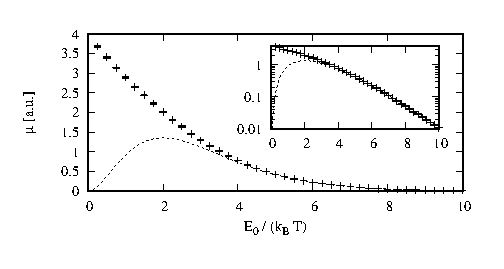
\includegraphics[width=\linewidth]{mu_vs_E0.eps}
  \caption{\label{mu_vs_E0}Escape rate versus $\frac{E_0}{k_BT}$ for
           $\frac{D}{R^2} = 1$. Points represent simulation results. The dotted
           line follows $\frac{5}{2}\left(\frac{E_0}{k_BT}\right)^2
           e^{-\frac{E_0}{k_BT}}$. The inset plots the same data points, but
           with a logarithmic scale on the vertical axis.}
\end{figure}


\section{Theoretical considerations}

The final step in this small project investigates the shape of function $f$ in
Eq. (\ref{dimensional_analysis}) following the classical approach by Kramers
\cite{Kramers1940}. First we imagine a one-dimensional setting with a potential
symmetrical about the origin $r = 0$, so that $V(-r) = V(r)$. Simply applying
Kramer's formula for the escape rate (taken from \cite{Escape_rate} without much
reflection) gives
\begin{align}
  \mu & = 2 \frac{D}{2 \pi k_BT} \sqrt{V''(0)\ |V''(R)|}
            e^{-\frac{E_0}{k_BT}} \nonumber \\
      & = \frac{6 D E_0}{\pi R^2 k_BT} e^{-\frac{E_0}{k_BT}}.
\end{align}

The extra factor of two in front comes from the two exits from the trap (at
$r = R$ and $r = -R$). Simulations suggest this factor should in fact be three
instead. Perhaps this emerges from a discontinuity of $V''$ at $r = R$? Whatever
the reason, the figure confirms a decay proportional to
$\frac{E_0}{k_BT} \exp\left(-\frac{E_0}{k_BT}\right)$ (Fig. \ref{mu_vs_E0_1D}).

\begin{comment}
%! codefile: mu_vs_E0_1D.gnuplot
set term postscript eps enhanced size 8cm,4cm font "Roman"
set output "mu_vs_E0_1D.eps"
set ylabel "{/Symbol m} [a.u.]"
set xlabel "E_0 / (k_B T)"

mu(x) = 2.82*x*exp(-x)

set multiplot
plot [0:10][0:2] "mu_vs_E0_1D.dat" u 1:5:6 w errorbars notitle lc -1, \
                 mu(x) w l dt 2 lc -1 notitle
set size 0.55, 0.55
set origin 0.4, 0.4
set logscale y
unset xlabel
unset ylabel
plot [0:10][:4] "mu_vs_E0_1D.dat" u 1:5:6 w errorbars notitle lc -1, \
                 mu(x) w l dt 2 lc -1 notitle
unset multiplot
%! codeend
\end{comment}

\begin{figure}
  \centering
  \includegraphics[width=\linewidth]{mu_vs_E0_1D.eps}
  \caption{\label{mu_vs_E0_1D}Escape rate versus $\frac{E_0}{k_BT}$ for
           $\frac{D}{R^2} = 1$ in the one-dimensional version of the problem.
           Simulation results are drawn with points. The dotted line follows
           $2.82\ \left(\frac{E_0}{k_BT}\right) e^{-\frac{E_0}{k_BT}}$.
           The inset shows the points on a logarithmic scale on the vertical
           axis.}
\end{figure}

\begin{comment}


The data sort of fits the expression
mu(x) = 2.4*x**2*exp(-x) + 5*exp(-x), where x = E/(k_BT).

 The probability distribution for the position of our
Brownian particle obeys the Smoluchowski equation.
\begin{equation}
  \frac{\partial P(\mathbf{r}, t | \mathbf{r}_0, t_0)}{\partial t}
    = \nabla \cdot \left(D\nabla - \frac{D}{k_BT} \mathbf{F}(\mathbf{r})\right)
                      P(\mathbf{r}, t | \mathbf{r}_0, t_0)
    = -\nabla \cdot \mathbf{J}(\mathbf{r}, t | \mathbf{r}_0, t_0).
\end{equation}
The vector field $\mathbf{J}$ is known as the probability \textit{flux}. The
problem becomes simpler once we assume that the particle starts at the origin
(as in the simulation) and that the potential is radially symmetrical, reducing
the study of $P(\mathbf{r}, t | \mathbf{r}_0, t_0)$ to $P(r, t | 0, 0)$, which
we write simply as $P(r, t)$. The distribution will not reach equilibrium
because probability will keep leaking out of the trap, but suppose that this
happens slowly enough that Boltzmann's equilibrium formula approximates the
distribution well enough. Then, because probability leaks out very slowly,
\begin{equation}
  \frac{\partial P(\mathbf{r}, t)}{\partial t} \approx 0,
\end{equation}
and the flux must depend very weakly on $r$ ($\nabla \cdot J \approx 0$). The
rate $\mu$ at which particles escape the trap equals the probability flowing
through the boundary of the trap at $r = R$. As we argued before, the vector
field $\mathbf(J)$ points radially outward and its modulus $J$ depends very
weakly on $r$, so
\begin{equation}
  \mu = \oint_{r = R} J dl = 2 \pi J R.
\end{equation}

We rewrite the flux in a form more convenient for our purposes here
\begin{equation}
  \mathbf{J} = -D e^{-\frac{V(r)}{k_BT}}\ 
               \nabla\left(e^{\frac{V(r)}{k_BT}} P(r, t)\right).
\end{equation}
If we were to approximate $P(r, t)$ by means of the Boltzmann distribution,
\begin{equation}
  \label{Boltzmann_distribution}
  P(r, t) \approx \frac{1}{N}e^{-\frac{V(r)}{k_BT}},
\end{equation}
then all we would get is $\mathbf{J} \approx \mathbf{0}$. Not much new
information there. However, if we rewrite the equation for $\mathbf{J}$ as
\begin{equation}
  \frac{\mathbf{J}}{D} e^{\frac{V(r)}{k_BT}}
    = \nabla\left(e^{\frac{V(r)}{k_BT}} P(r, t)\right),
\end{equation}
and integrate over the trap area on both sides, we may conclude that
\begin{equation}
  \label{J_integrals}
  \mathbf{J}
    = D \frac{\int_0^R \frac{d}{dr}\left(e^{\frac{V(r)}{k_BT}}
                                         P(r, t)\right)\ r\ dr}
             {\int_0^R e^{\frac{V(r)}{k_BT}}\ r\ dr}.
\end{equation}
The numerator we integrate by parts.
\begin{equation}
  \int_0^R \frac{d}{dr}\left(e^{\frac{V(r)}{k_BT}} P(r, t)\right)\ r\ dr
    = \left[e^{\frac{V(r)}{k_BT} P(r, t)\ r}\right]_0^R
      - \int_0^R e^{\frac{V(r)}{k_BT}} P(r, t)\ dr.
\end{equation}
The first term on the right vanishes at $r = 0$ and we neglect its value at
$r = R$ because $P(R, t) \approx 0$. To solve the integral on the right we use
the approximation (\ref{Boltzmann_distribution}).
\begin{equation}
  -\int_0^R e^{\frac{V(r)}{k_BT}} \frac{1}{N} e^{-\frac{V(r)}{k_BT}}\ dr
     = -\frac{R}{N}.
\end{equation}
The denominator in Eq. (\ref{J_integrals}) allows for a series approximation.
\begin{equation}
  \int_0^R e^{\frac{V(r)}{k_BT}}\ r\ dr
    \approx R^2 e^{-\frac{E_0}{k_BT}}\left(\frac{1}{2}
                   + \frac{7 E_0}{20 k_BT}\right).
\end{equation}

Series expansion of the integral at $r = 0$:
https://www.wolframalpha.com/input/?i=integrate+exp%28E_0*%28-2*%28r%2FR%29%5E3+%2B+3*%28r%2FR%29%5E2+-+1%29%2F%28k*T%29%29+r+dr
\end{comment}

\begin{thebibliography}{9}

\bibitem{Kramers1940} \textsc{H.~A.~Kramers}, \textit{Brownian motion in a field
of force and the diffusion model of chemical reactions}, Physica \textbf{7}, 4,
284--304 (1940).

\bibitem{Escape_rate} \url{https://home.icts.res.in/\~abhi/notes/kram.pdf}.


\end{thebibliography}

\end{document}

%%%%%%%%%%%%%%%%%%%%%%%%%%%%%%%%%% Makefile %%%%%%%%%%%%%%%%%%%%%%%%%%%%%%%%%%%%

%! codefile: Makefile
all: tangle code data figures weave

tangle:
	txt2tangle kramers.tex

code:
	gcc -Wall -march=native -Ofast -lm -o cubic_spline cubic_spline.c

data:
	bash cubic_spline.sh

figures:
	gnuplot cubic_spline.gnuplot
	gnuplot mu_vs_D_and_R.gnuplot
	gnuplot mu_vs_E0.gnuplot
	gnuplot mu_vs_E0_1D.gnuplot

weave:
	latex kramers.tex
	dvips kramers.dvi
	ps2pdf kramers.ps
%! codeend

%! codefile: README.md

# Escape rate for a Brownian particle in a radial cubic spline trap

%! codeinsert: introduction

## Aim

This short project illustrates literate programming using the **txt2tangle**
tool. You can check out the final result in the **kramers.pdf** file.

## Compiling and running

This project assumes that your system has the following tools installed:
**txt2tangle**, **make**, **gcc**, **bash**, **gnuplot**, **latex**, **dvips**
and **ps2pdf**. *All* the files for this project (including this one) stem from
**kramers.tex**. By running `txt2tangle kramers.tex`, you can generate the
`Makefile`. Everything else in the project (compiling, running and outputting
the final report) takes place when you execute `make`.

%! codeend

%! codefile: random.h
# ifndef _RANDOM_H_
# define _RANDOM_H_

# ifndef ONLY_PREPROCESSOR
# include <stdint.h>
# else
//!# include <stdint.h>
# endif

# ifndef __bool_type__
# define __bool_type__
typedef enum {false, true} bool; /* Boolean type */
# endif

/* Pseudorandom number generation */
uint64_t s[] = {12679825035178159220ull, 15438657923749336752ull}; /* PRNG seed */

# ifdef PRNG_XORSHIFT
# define PRNG() xorshift128plus()
# define RANDOM_MAX 18446744073709551615ull
/* 64-bit (pseudo)random integer */
uint64_t xorshift128plus(void)
{
  uint64_t x = s[0];
  uint64_t const y = s[1];
  s[0] = y;
  x ^= x << 23; // a
  x ^= x >> 17; // b
  x ^= y ^ (y >> 26); // c
  s[1] = x;
  return x + y;
}
# else
/* Minimal PCG32 code adapted from M.E. O'Neill: pcg-random.org (2014) */
# define PRNG() pcg32_random_r()
# define RANDOM_MAX 4294967295ul

uint32_t pcg32_random_r(void)
{
    uint64_t oldstate = s[0];
    // Advance internal state
    s[0] = oldstate * 6364136223846793005ULL + (s[1]|1);
    // Calculate output function (XSH RR), uses old state for max ILP
    uint32_t xorshifted = ((oldstate >> 18u) ^ oldstate) >> 27u;
    uint32_t rot = oldstate >> 59u;
    return (xorshifted >> rot) | (xorshifted << ((-rot) & 31));
}
# endif

/* Random number from a uniform distribution */
double uniform(double min, double max)
{
  return min + (PRNG()/((double) RANDOM_MAX))*(max - min);
}

# ifndef NO_GAUSSIAN_PRNG
/* Random number from a Gaussian distribution */
float Gaussian(float mean, float stddev)
{
  double u1, u2, s0 = 2;
  static bool saved_value = false; /* Flag indicating stored number */
  static double Gnum; /* Stored Gaussian number */

  if(saved_value) {
    saved_value = false;
    return Gnum;
  }

  while(s0 >= 1)
  {
    u1 = uniform(-1, 1);
    u2 = uniform(-1, 1);
    s0 = u1*u1 + u2*u2;
  }

  Gnum = mean + stddev*u2*sqrt(-2*logf(s0)/s0);
  saved_value = true;

  return mean + stddev*u1*sqrt(-2*logf(s0)/s0);
}
# endif

/* Marsaglia's algorithm for random point on a unit sphere */
void random_axis(float * n)
{
  float x, y, s = 2;

  while(s > 1) {
    x = uniform(-1, 1);
    y = uniform(-1, 1);
    s = x*x + y*y;
  }

  n[0] = 2*x*sqrt(1 - s);
  n[1] = 2*y*sqrt(1 - s);
  n[2] = 1 - 2*s;

  return;
}

/* To change the PRNG seed you may use code like this:
// The PRNG state must be seeded so that it is not everywhere zero.
s[0] = 12679825035178159220u;
s[1] = 15438657923749336752u;
*/

# endif
%! codeend
